\documentclass[12pt, titlepage]{article}

\usepackage{xcolor} % for different colour comments
\usepackage{hyperref}
\hypersetup{
    colorlinks,
    citecolor=black,
    filecolor=black,
    linkcolor=red,
    urlcolor=blue
}
\usepackage{graphicx}
\graphicspath{ {image/} }

%% Comments
\newif\ifcomments\commentstrue

\ifcomments
\newcommand{\authornote}[3]{\textcolor{#1}{[#3 ---#2]}}
\newcommand{\todo}[1]{\textcolor{red}{[TODO: #1]}}
\else
\newcommand{\authornote}[3]{}
\newcommand{\todo}[1]{}
\fi

\newcommand{\wss}[1]{\authornote{magenta}{SS}{#1}}
\newcommand{\ds}[1]{\authornote{blue}{DS}{#1}}

\begin{document}

\title{\bf Physics-Based Chipmunk2D Game\\[\baselineskip]\Large Proof of Concept Demonstration Plan}
\author{Steven Palmer\\$\langle$palmes4$\rangle$\\Emaad Fazal\\$\langle$fazale$\rangle$\\Chao Ye\\$\langle$yec6$\rangle$}
\date{\today}
	
\maketitle

\section*{Significant Risks}
The successful completion of the project depends on overcoming the following significant risks:
\begin{enumerate}
  \item In order to use the Chipmunk2D library it must first be successfully compiled.  Since we intend for the game to be compatible with Windows 7, Mac OS X, and Ubuntu, there is a significant risk for the project to fail if compilation is not achieved on all three operating systems.
  \item Chipmunk2D is a large library and its use is not straight forward.  Successful implementation of the library features is crucial to the success of the project and the failure of this poses another significant risk.
\end{enumerate}


\section*{Demonstration Plan}

For our proof of concept demonstration we will produce a working prototype that supports the operating systems mentioned above.  The prototype will consist of a game demo that implements gravity and collision detection provided by the Chipmunk2D library.  Rudimentary graphics will be used for the prototype since the scope is limited only to demonstrating that the identified risks can be overcome.

The prototype will consist of a small room in which a hero character and enemies exist.  The room will be bounded by a floor below and walls on the left and right, all of which the hero and enemies cannot pass through.  The room will contain platforms which the hero and enemies cannot pass through from above, but may pass through from below when jumping.  A rough idea of the room is given in \hyperref[fig:room]{Figure~\ref*{fig:room}}.

\begin{figure}[hB]
\begin{center}
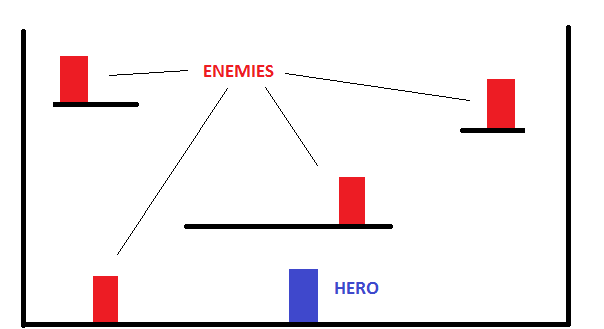
\includegraphics[width=0.75\textwidth]{demo}
\caption{Sketch of room} \label{fig:room}
\end{center}
\end{figure}

The hero character will be represented by a blue rectangle and will be controlled by the user in the following ways:

\begin{itemize}
  \item The hero moves left and right using the 'a' and 'd' keys respectively
  \item The hero jumps by pressing the 'space' key
  \item The hero shoots a projectile in the direction of the mouse cursor by left-clicking
\end{itemize}

Enemies will be represented by red rectangles and will not have any programmed AI (they will not move or attack).  The hero will be able to attack enemies with a projectile, which will knock them back when they are hit.  The hero and all enemies will be subject to gravity and will free-fall when there is no platform or boundary under them.

\end{document}
